% THIS TEMPLATE IS A WORK IN PROGRESS

\documentclass{article}
\usepackage{graphicx}
\usepackage{hyperref}
\usepackage{fancyhdr}
\usepackage{float}
\usepackage{hyperref}

% FOR CODE
\usepackage{listings}
\usepackage{xcolor}
\usepackage{xparse}
\NewDocumentCommand{\codeword}{v}{%
\texttt{{#1}}%
}

\definecolor{codegreen}{rgb}{0,0.6,0}
\definecolor{codegray}{rgb}{0.5,0.5,0.5}
\definecolor{codepurple}{rgb}{0.58,0,0.82}
\definecolor{backcolour}{rgb}{0.95,0.95,0.92}

\lstdefinestyle{mystyle}{
    backgroundcolor=\color{backcolour},   
    commentstyle=\color{codegreen},
    keywordstyle=\color{magenta},
    numberstyle=\tiny\color{codegray},
    stringstyle=\color{codepurple},
    basicstyle=\ttfamily\footnotesize,
    breakatwhitespace=false,         
    breaklines=true,                 
    captionpos=b,                    
    keepspaces=true,                 
    numbers=left,                    
    numbersep=5pt,                  
    showspaces=false,                
    showstringspaces=false,
    showtabs=false,                  
    tabsize=2
}

\lstset{style=mystyle}
% 

\fancypagestyle{firstpage}{%
  \lhead{CAP6610 Project Progress Report}
  \rhead{Akash Gajjar}
}

\begin{document}
\thispagestyle{firstpage}

\section{Summary}

Even though I was not able to fully understand the mathematics behind the VAE, I understood how the model should be set up so that I am able to train the VAE on MNIST dataset and generate some hand written digits. I also found that \codeword{pytorch} has a \codeword{datasets} class which contains standard data loaders for various datasets so I used that one instead of my custom data loader since it would be more compatible with \codeword{pytorch}. I was able to implement the VAE using \codeword{pytorch} and taking some help from \codeword{stackoverflow}. I am generating the samples from 20-D latent space. Given that, My model has the following architecture $784 \rightarrow 400 \rightarrow 200 \rightarrow 20 \rightarrow 200 \rightarrow 400 \rightarrow 784$. The appendix in the paper \cite{1} was helpful in clearing out some confusion as well. I trained the model on training data for 30 epochs, 128 batch size, and $10^{-3}$ learning rate. Also, I used ReLU activation function and adam optimizer as I found that these make the network converge faster. For loss, I used Binary Cross Entropy + KL term (as indicated in Appendix B of the paper \cite{1}). Initially I used only BCE loss but the generated samples were not hand written digit-like at all. So I had to look up on the internet about the loss function of VAE.

\section{Model Code}

\begin{lstlisting}[language=Python]
class VAE(nn.Module):
    def __init__(self):
        super(VAE, self).__init__()

        self.fc1 = nn.Linear(784, 400)
        self.fc2 = nn.Linear(400, 200)
        self.fc31 = nn.Linear(200, 20)
        self.fc32 = nn.Linear(200, 20)
        self.fc4 = nn.Linear(20, 200)
        self.fc5 = nn.Linear(200, 400)
        self.fc6 = nn.Linear(400, 784)

    def encode(self, x):
        h1 = F.relu(self.fc1(x))
        h2 = F.relu(self.fc2(h1))
        return self.fc31(h2), self.fc32(h2)

    def reparameterize(self, mu, logvar):
        std = torch.exp(0.5 * logvar)
        eps = torch.randn_like(std)
        return mu + eps * std

    def decode(self, z):
        h3 = F.relu(self.fc4(z))
        h4 = F.relu(self.fc5(h3))
        return torch.sigmoid(self.fc6(h4))

    def forward(self, x):
        mu, logvar = self.encode(x.view(-1, 784))
        z = self.reparameterize(mu, logvar)
        return self.decode(z), mu, logvar
\end{lstlisting}

\section{Generated Samples}
Here are some generated samples from epoch 1 and epoch 30

\begin{figure}[H]
  \centering
  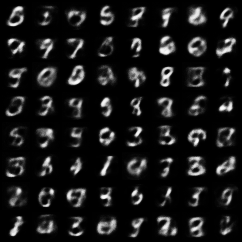
\includegraphics[width=2in]{src/results/sample_1.png}
  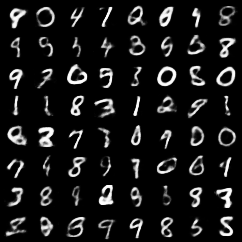
\includegraphics[width=2in]{src/results/sample_30.png}
  \caption{Epoch 1 and Epoch 30}
\end{figure}
We can clearly see that the features of the digits are much sharper after training for 30 epochs. The loss at the start of the training was 183 and towards the end of training it was reduced to 99.

\section{Next Steps}

Now that I am able to generate some samples from the VAE, I would like to do the same for GAN as well (I am able to generate some samples from GAN but they are not good). After successfully generating the samples from both, I would like to compare those samples and see which model is better in terms of training required and convergence time. In parallel, I would like to improve my fundamental understanding of GAN and VAE by reading more about it.

\begin{thebibliography}{1}

\bibitem{1} \url{https://arxiv.org/pdf/1312.6114.pdf}

\end{thebibliography}

\end{document}
